\begin{frame}{\fttheory{Interest Rate Swaps}}
    \begin{itemize}
        \item The Solomon swap was a \textit{currency} swap
        \item We will start with \textit{interest rate} swaps
        \item A vanilla swap is ``fixed-for-floating''
        \item The party who is long the swap receives fixed rate cash flows and pays floating rate cash flows 
    \end{itemize}
\end{frame}

\begin{frame}{\fttheory{Interest Rate Swaps}}
    \begin{center}
        \begin{tabular}{lcc}
            Term & Year $0$ & Year $1$ \\ \hline
            One-Year & $_{0}y_{1}$ & $_{1}y_{1}$ \\
            Two-Year & $_{0}y_{2}$ & $\times$
        \end{tabular}
    \end{center}
    \begin{itemize}
        \item Suppose we have the above yield curve
        \item All bonds on the yield curve are 1k, zero-coupon
        \item There are two kinds of loans, fixed and floating
        \item Fixed loan: borrow with \underline{known} coupons $_{0}c_{2}\equiv\:_{0}y_{2}\cdot 1$k in years one and two 
        \item Floating loan: borrow with \underline{known} coupon $_{0}c_{1}\equiv\:_{0}y_{1}\cdot 1$k in the year one and \underline{unknown} coupon $_{1}c_{1}\equiv\:_{1}y_{1}\cdot 1$k in year two
    \end{itemize}
\end{frame}

\begin{frame}{\fttheory{Interest Rate Swaps}}
    \begin{itemize}
        \item Consider two firms, $A$ and $B$
        \item $A$ makes fixed payments on its debt
        \item $B$ makes floating payments on its debt
    \end{itemize}
\begin{center}
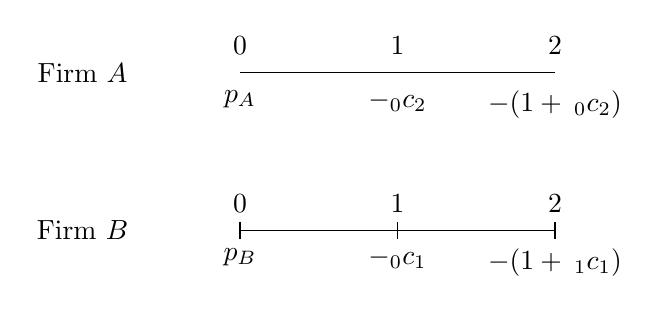
\begin{tikzpicture}
    
    \draw (0,0) -- (4,0);
    \foreach \x in {0,2,4}
    \draw(\x cm,3pt) -- (\x cm, -3pt);
    \draw (0,0) node[above=3pt] {0};
    \draw (2,0) node[above=3pt] {1};
    \draw (4,0) node[above=3pt] {2};
    \draw (-2,0) node[] {Firm $B$};
    \draw (0,0) node[below=3pt] {$p_{B}$};
    \draw (2,0) node[below=3pt] {$-_{0}c_{1}$};
    \draw (4,0) node[below=3pt] {$-(1+\:_{1}c_{1})$};
    
    \draw (0,2) -- (4,2);
    \foreach \x in {0,2,4}
    \draw(\x cm,3pt) -- (\x cm, -3pt);
    \draw (0,2) node[above=3pt] {0};
    \draw (2,2) node[above=3pt] {1};
    \draw (4,2) node[above=3pt] {2};
    \draw (-2,2) node[] {Firm $A$};
    \draw (0,2) node[below=3pt] {$p_{A}$};
    \draw (2,2) node[below=3pt] {$-_{0}c_{2}$};
    \draw (4,2) node[below=3pt] {$-(1+\:_{0}c_{2})$};
\end{tikzpicture}
\end{center}
\end{frame}

\begin{frame}{\fttheory{Interest Rate Swaps}}
    \begin{itemize}
        \item If we assume that the original debts were priced correctly, 
            \begin{equation}
                p_{A}=p_{B}=1
            \end{equation}
        \item Coupon rate always equals yield, so bond always worth face
        \item You can show this with a no-arbitrage argument
    \end{itemize}
\end{frame}

\begin{frame}{\fttheory{Interest Rate Swaps}}
    \begin{itemize}
        \item $A$ \underline{makes} fixed payments and \underline{wants} floating payments
        \item $B$ \underline{makes} floating payments and \underline{wants} fixed payments
        \item Solution: $A$ sells a swap to $B$ 
    \end{itemize}
\end{frame}

\begin{frame}{\fttheory{Interest Rate Swaps}}
    $W_{0}$ is the price of the swap
    \begin{center}
        \begin{tabular}{lcccc}
            Security & Q & CF$_{0}$ & CF$_{1}$ & CF$_{2}$\\ \hline
            \multicolumn{5}{c}{\textbf{Firm A}} \\ \hline
            Loan (Fixed) & $+1$ & $+p_{A}$ & $-\:_{0}c_{2}$ & $-(1+\:_{0}c_{2})$\\
            Swap & $+1$ & $-w_{0}$ & $_{0}c_{2}-\:_{0}c_{1}$ & $_{0}c_{2}-\:_{1}c_{1}$ \\ \hline
            & & $p_{A}-w_{0}$ & $-\:_{0}c_{1}$ & $-(1+\:_{1}c_{1}$) \\ \hline
            \multicolumn{5}{c}{\textbf{Firm B}} \\ \hline
            Loan (Floating) & $+1$ & $+p_{B}$ & $-\:_{0}c_{1}$ & $-(1+\:_{1}c_{1})$ \\
            Swap & $-1$ & $+w_{0}$ & $-(_{0}c_{2}-\:_{0}c_{1})$ & $-(_{0}c_{2}-\:_{1}c_{1})$ \\ \hline
            & & $p_{B}+w_{0}$ & $-\:_{0}c_{2}$ & $-(1+\:_{0}c_{2})$
        \end{tabular}
    \end{center}
    $A$'s payments are now floating and $B$'s payments are now fixed
\end{frame}

\begin{frame}{\ftexampl{Interest Rate Swaps}}
    \begin{itemize}
        \item The rate on two-year debt is 10\% this year
        \item The rate on one-year debt is 10\% this year, but the rate on one-year debt could either be 5\% or 15\% next year. 
    \end{itemize}
    \begin{center}
        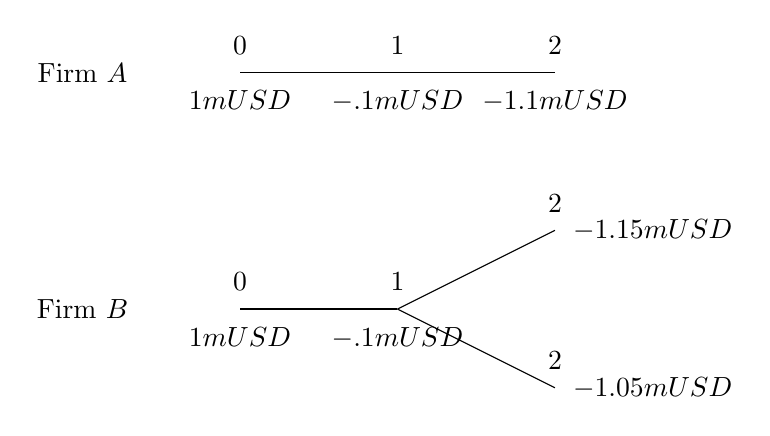
\begin{tikzpicture}

            \draw (0,3) -- (4,3);
            \draw (-2,3) node[] {Firm $A$};
            \draw (0,3) node[above=3pt] {0};
            \draw (2,3) node[above=3pt] {1};
            \draw (4,3) node[above=3pt] {2};
			\draw (0,3) node[below=3pt] {$1\text{m USD}$};
			\draw (2,3) node[below=3pt] {$-.1\text{m USD}$};
			\draw (4,3) node[below=3pt] {$-1.1\text{m USD}$};
            
            \draw (0,0) -- (2,0);
            \draw (2,0) -- (4,1);
            \draw (2,0) -- (4,-1);
            \draw (-2,0) node[] {Firm $B$};
            \draw (0,0) node[above=3pt] {0};
            \draw (2,0) node[above=3pt] {1};
            \draw (4,1) node[above=3pt] {2};
            \draw (4,-1) node[above=3pt] {2};
			\draw (0,0) node[below=3pt] {$1\text{m USD}$};
			\draw (2,0) node[below=3pt] {$-.1\text{m USD}$};
			\draw (4,1) node[right=3pt] {$-1.15\text{m USD}$};
			\draw (4,-1) node[right=3pt] {$-1.05\text{m USD}$};
        \end{tikzpicture}
    \end{center}
\end{frame}

\begin{frame}{\ftexampl{Interest Rate Swaps}}
    Suppose that $w_{0}=0$. Units are millions of USD.
    \begin{center}
        \begin{tabular}{lccccc}
            Security & Q & CF$_{0}$ & CF$_{1}$ & CF$_{2,u}$ & CF$_{2,d}$\\ \hline
            \multicolumn{6}{c}{\textbf{Firm A}} \\ \hline
            Loan (Fixed) & $+1$ & $+1$ & $-.1$ & $-1.1$ & $-1.1$ \\
            Swap & $+1$ & $0$ & $0$ & $-.05$ & $+.05$ \\ \hline
            & & $+1$ & $-.1$ & $-1.15$ & $-1.05$\\ \hline
            \multicolumn{6}{c}{\textbf{Firm B}} \\ \hline
            Loan (Floating) & $+1$ & $+1$ & $-.1$ & $-1.15$ & $-1.05$ \\
            Swap & $-1$ & $0$ & $0$ & $+.05$ & $-.05$ \\ \hline
            & & $+1$ & $-.1$ & $-1.1$ & $-1.1$
        \end{tabular}
    \end{center}
    $A$'s payments are now floating and $B$'s payments are now fixed
\end{frame}

\begin{frame}{\fttheory{Interest Rate Swaps: Pricing}}
    $w_{0}$ is the price of the swap
    \begin{center}
        \begin{tabular}{lcccc}
            Security & Q & CF$_{0}$ & CF$_{1}$ & CF$_{2}$\\ \hline
            Swap & $+1$ & $-w_{0}$ & $_{0}c_{2}-\:_{0}c_{1}$ & $_{0}c_{2}-\:_{1}c_{1}$ \\ \hline
            \multicolumn{5}{c}{Replicating Portfolio} \\ \hline
            $_{0}c_{2}$ & $+1$ & $-1$ & $_{0}c_{2}$ & $1+\:_{0}c_{2}$ \\
            $_{0}c_{1}$ & $-1$ & $+1$ & $-(1+\:_{0}c_{1})$ & $\times$ \\
            $_{1}c_{1}$ & $-1$ & $\times$ & $+1$ & $-(1+\:_{1}c_{1})$\\ \hline
            & & $0$ & $_{0}c_{2}-\:_{0}c_{1}$ & $_{0}c_{2}-\:_{1}c_{1}$
        \end{tabular}
    \end{center}
    Absent arbitrage, $w_{0}=0$. 
\end{frame}

\iffalse

\begin{frame}{Interest Rate Swaps: Arbitrage (Long)}
    $W_{0}$ is the price of the swap
    \begin{center}
        \begin{tabular}{lcccc}
            Security & Q & CF$_{0}$ & CF$_{1}$ & CF$_{2}$\\ \hline
            Swap & $+1$ & $-w_{0}$ & $_{0}c_{2}-\:_{0}c_{1}$ & $_{0}c_{2}-\:_{1}c_{1}$ \\
            $_{0}c_{2}$ & $+1$ & $-_{0}p_{2}$ & $_{0}c_{2}$ & $1+\:_{0}c_{2}$ \\
            $_{0}c_{1}$ & $-1$ & $+1$ & $-(1+\:_{0}c_{1})$ & $\times$ \\
            $_{1}c_{1}$ & $-1$ & $\times$ & $+1$ & $-(1+\:_{1}c_{1})$ \\ \hline 
            & & $1-\:_{0}p_{2}$ & $0$ & $0$
        \end{tabular}
    \end{center}
\end{frame}

\begin{frame}{Interest Rate Swaps: Arbitrage (Short)}
    $W_{0}$ is the price of the swap
    \begin{center}
        \begin{tabular}{lcccc}
            Security & Q & CF$_{0}$ & CF$_{1}$ & CF$_{2}$\\ \hline
            Swap & $+1$ & $-w_{0}$ & $_{0}c_{2}-\:_{0}c_{1}$ & $_{0}c_{2}-\:_{1}c_{1}$ \\
            $_{0}c_{2}$ & $+1$ & $-_{0}p_{2}$ & $_{0}c_{2}$ & $1+\:_{0}c_{2}$ \\
            $_{0}c_{1}$ & $-1$ & $+1$ & $-(1+\:_{0}c_{1})$ & $\times$ \\
            $_{1}c_{1}$ & $-1$ & $\times$ & $+1$ & $-(1+\:_{1}c_{1})$ \\ \hline 
            & & $1-\:_{0}p_{2}$ & $0$ & $0$
        \end{tabular}
    \end{center}
\end{frame}

\begin{frame}{Board Problem 1}
    Suppose that the yield on a one-year bond is 5\% ($_{0}y_{1}=5\%$) and the yield on a two-year bond is 10\% ($_{0}y_{2}=10\%$). What should the swap trade for ($w_{0}$)? What if it trades for \$1m? What if trades for \$2m? 
\end{frame}

\fi
